


\section{Conceptos básicos de regulación genética}

% Inducción, Represión catabólica, Represor, Regulador, Inductor, Gen promotor, Operador

\section{Operones}

Los operones son grupos de genes los cuales tienen una expresión regulada, esto para evitar transcripciones indeseadas, como una producción de ácido clorhídrico (HCl) en tejidos no estomacales o la producción de enzimas no necesarias en ese momento, entre otros ejemplos. Estos operones están regulados por elementos de control, como un promotor y/o un operador, además de un gen regulador.

El control de la expresión génica dado en los operones puede ser positivo o negativo.

\begin{itemize}
    \item Positvo: Lo es cuando el producto del gen regulador activa la expresión de los genes, actuando como activador.
    \item Negativo: Lo es cuando el producto del gen regulador reprime la expresión génica, actuando como represor.
\end{itemize}

El orden general de los operones es:

\begin{enumerate}
    \item Gen y proteína reguladores
    \item Promotor
    \item Operador: Sitio en el que se situa la proteína reguladora.
    \item Genes estructurales: Genes regulados
\end{enumerate}

\section{Operones de control positivo y de control negativo}



\section{Ejemplos de operones}

\subsection{Operón LAC}

Un ejemplo de operón es el operón Lac, encontrado en algunas bacterias. Este que actua de la siguiente manera:

\begin{enumerate}
    \item Sin lactosa
        \begin{figure}[H]
            \centering
            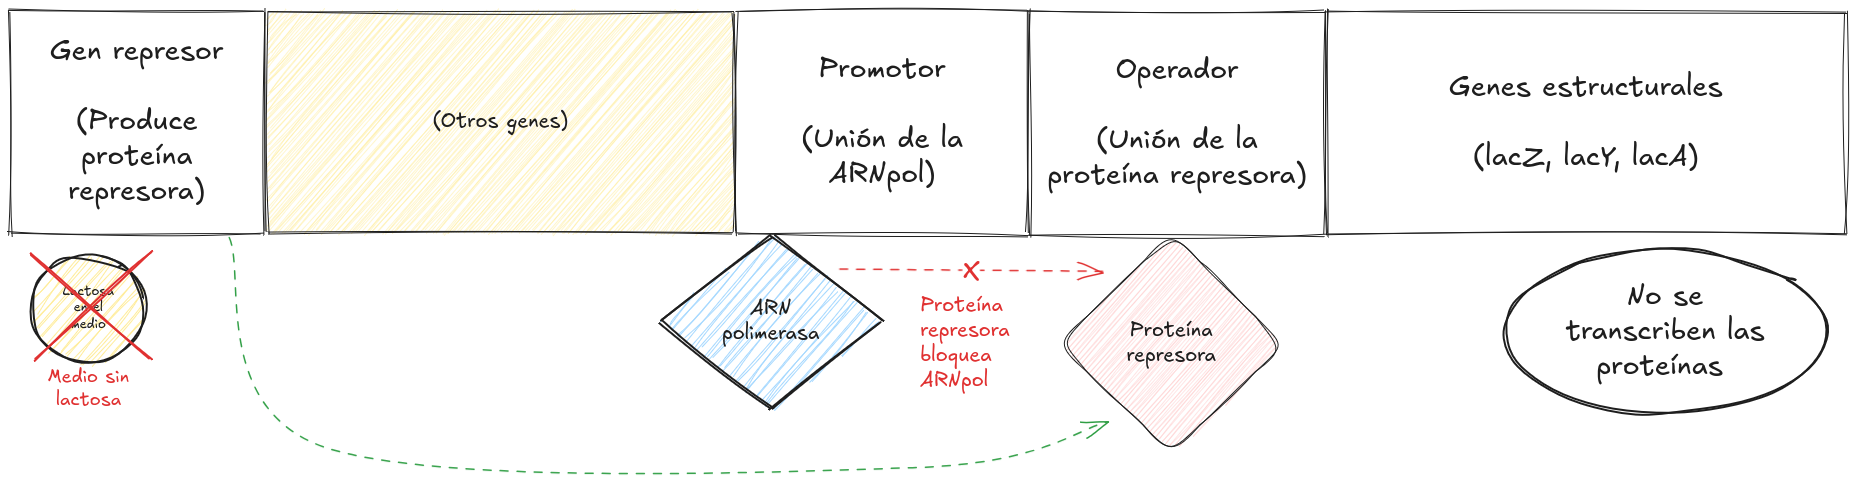
\includegraphics[width=0.85\textwidth]{./images/Operón_LAC_sin_lactosa.png}
            \caption{Operón LAC sin lactosa}
            \label{fig:Operón_LAC_sin_lactosa}
        \end{figure}
    
    \item Con lactosa
        \begin{figure}[H]
            \centering
            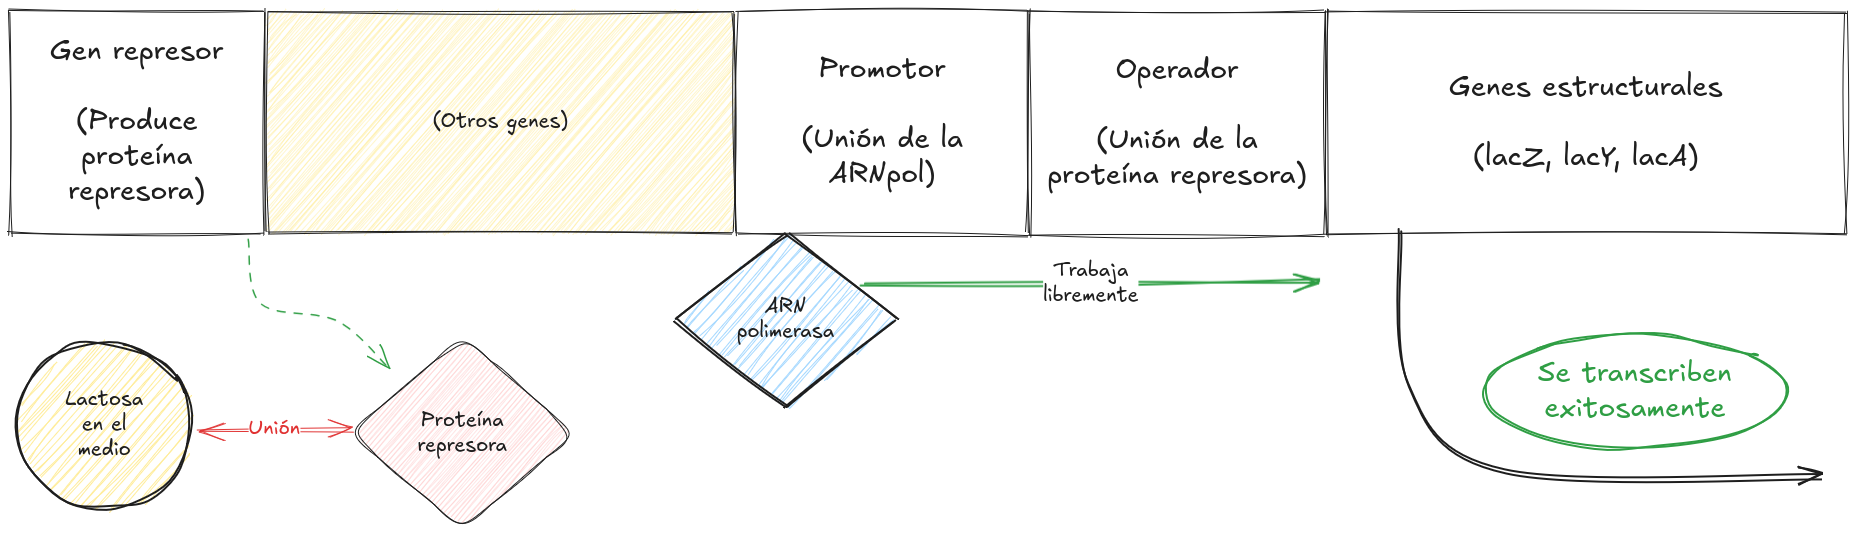
\includegraphics[width=0.85\textwidth]{./images/Operón_LAC_con_lactosa.png}
            \caption{Operón LAC con lactosa}
            \label{fig:Operón_LAC_con_lactosa}
        \end{figure}
\end{enumerate}

Como se aprecia en la \autoref{fig:Operón_LAC_sin_lactosa}, la unión de la proteína represora al operador bloquea a la ARNpol e impide la transcripción de los genes estructurales (lacZ, lacY y lacA). El funcionamiento es diferente si hay lactosa en el medio, pues la lactosa se une a la proteína represora y permite que la ARNpol avanze por la hebra de ADN y realize la transcipción de los genes estructurales.

Así pues, este es un operón que funciona bajo control negativo, esto porque la proteína represora se une al operador en la ausencia del inductor, que en este caso se denominaría activador, pues su presencia activa el procesamiento de los genes estructurales.

Los genes estructurales dan lugar a proteínas que están involucradas en el metabolismo de la lactosa, por lo que la síntesis de estas proteínas disminuye los niveles de lactosa hasta que no se bloquea más a la proteína represora, detendiendo de nuevo la síntesis de genes estructurales. Este sistema entonces funciona como un ``interruptor'' que activa la capacidad de la bacteria de metabolizar lactosa cuando esta está presente en el medio, mientras que la desactiva cuando no existe para así no sintetizar proteínas que no serán utilizadas.

\subsection{Operón triptófano}

Otro ejemplo de operón es el operón trp, encargado de regular la síntesis de triptófano. Este operón, sin embargo, es de control positivo. Este operón necesita de una molécula (el triptófano) para que al operador se una la proteína represora. Puesto que los genes estructurales se encargan de la síntesis de triptófano, este operón regula la sobreproducción de tal aminoácido.

\begin{enumerate}
    \item Sin triptófano
        \begin{figure}[H]
            \centering
            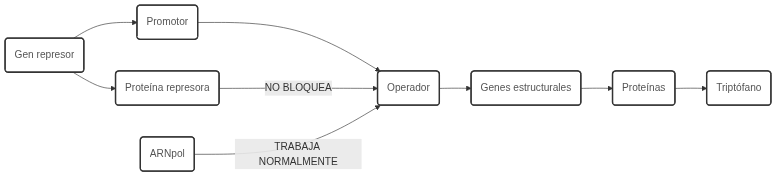
\includegraphics[width=0.85\textwidth]{./images/Operón_TRP_sin_triptófano.png}
            \caption{Operón triptófano sin triptófano}
            \label{fig:Operón_TRP_sin_triptófano}
        \end{figure}
    
    \item Con triptófano
        \begin{figure}[H]
            \centering
            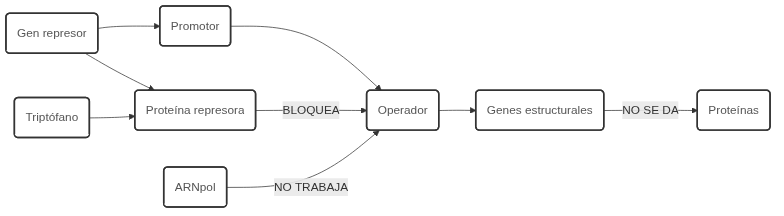
\includegraphics[width=0.85\textwidth]{./images/Operón_TRP_con_triptófano.png}
            \caption{Operón triptófano con triptófano}
            \label{fig:Operón_TRP_con_triptófano}
        \end{figure}
\end{enumerate}

\section{Regulones}



\section{Operones y regulones en organismos}



\section{Mecanismos de atenuación}



\section{Mecanismos de metilación y acetilación}

Para controlar la forma en que los genes de un organismo se expresan existen diversos mecanismos en las células para "decidir" qué genes están disponibles para la síntesis de proteínas y cuáles no. A esto se le conoce como regulacón de la expresión génica.

Como hemos visto, en procarioras existen los operones, pero estos no están presentes en eucariotas. En su lugar, existen otros mecanismos, los cuales pueden actuar en distintos niveles:

\begin{enumerate}
    \item Nivel cromatina (por acetilación)
    \item Regulación de factores de transcripción
    \item Procesamiento del ARN
    \item Estabilidad del ARN
    \item Nivel traducción
    \item Actividad de la proteína
\end{enumerate}

\subsection{Metilación}

Uno de los mecanismos de la regulación de la expresión génica es la metilación. Este proceso consiste en la adición de un grupo metilo al carbono 5 de la citosina, esto realizado por las ADN metiltransferasas. Este cambio en el ADN  provoca  que no sea posible "leer" el ADN, por lo que no se puede dar la expresión de tales genes.

\subsection{Acetilación}

Un proceso similar es la acetilación, donde se añade, en este caso, un grupo acetilo, sin embargo, el lugar de adición es en el as histonas, donde cumple la función de "relajar" las histonas y permitir la transcripción de genes. Las enzimas encargadas de esto son las histonas-deacetilasas.

\section{Epigenética}


